\chapter{Evaluation}
\label{sec:evaluation}

Chapters~\ref{sec:derivative-parser} and~\ref{sec:partial-derivative-parser}
developed four parser combinations, \texttt{deriv\_std} (recursive and
loop variants), \texttt{deriv\_bc}, \texttt{pderiv\_std} and
\texttt{pderiv\_bc}, each claimed to compute either the POSIX or the
leftmost-first parse tree, by four structurally different constructions.
This chapter evaluates those four parsers against each other, first for
correctness and then for performance, on two kinds of input: 1. Small,
constructed patterns taken from the source paper to isolate one
algorithmic property at a time; 2. A corpus of real-world regular
expressions assembled from three sources: Snort/Suricata,
SpamAssassin and RegexLib, that Mamouras et al.'s disambiguation-robustness
study \citep{mamouras2024} uses. 

That paper studies exactly the
POSIX-versus-Greedy question this thesis studies, via real intrusion-detection
signatures, and finds concrete real-world patterns where the two policies
visibly diverge. It provides no public dataset artifact of its own, so
Section~\ref{sec:dataset-preparation} describes how the 
corpus was independently assembled and prepared.

Section~\ref{sec:correctness-verification} checks the four parsers, and
the three Boolean matchers of Chapter~\ref{sec:derivatives}, against each
other and against the paper's own worked examples.
Section~\ref{sec:dataset-preparation} describes both input sources:
synthetic patterns and the real-world corpus.
Section~\ref{sec:performance-analysis} measures where the four parsers'
costs diverge on each and the final Section~\ref{sec:results-discussion} draws the
two together.

%
%
%

\section{Parser Agreement}
\label{sec:correctness-verification}

\paragraph{Paper A1 Example:.} 
$r_1 = (a + ab)(b + \varepsilon)$ and $w = \mathtt{ab}$,

\begin{figure}[htbp]
\small
\centering
\begin{verbatim}
$ cargo run -- parse "(a|ab)(b|)" "ab" --parser all
Parser       | Policy    | Result
-------------+-----------+-------------------------------
DERIV_REC    | POSIX     | (Right (a, b), Right ()) -> "ab"
DERIV_LOOP   | POSIX     | (Right (a, b), Right ()) -> "ab"
DERIV_BC     | POSIX     | (Right (a, b), Right ()) -> "ab"
PDERIV_STD   | NON-POSIX | (Left a, Left b) -> "ab"
PDERIV_BC    | NON-POSIX | (Left a, Left b) -> "ab"

POSIX parsers agree
PDERIV parsers agree
NON-POSIX agrees with POSIX on membership
\end{verbatim}
\caption{Comparison of the parser results for the regular expression $(a|ab)(b|)$.}
\label{fig:parser-comparison}
\end{figure}


\paragraph{Paper A2 Example:.} 
$r_2 = (a+b+ab)^{\ast}$ against $w=\mathtt{ab}$,

%
%
%

\section{Dataset Preparation}
\label{sec:dataset-preparation}

Two kinds of input drive the measurements in this chapter, and they are
kept deliberately distinct rather than pooled into one corpus.

\subsection{Synthetic Patterns}
\label{sec:synthetic-patterns}

The synthetic patterns used throughout this thesis, \texttt{paper\_r1},
\texttt{paper\_r2}, the pathological $(a^{*})^{*}$-style expressions of
Section~\ref{sec:membership-overview}, and the benchmark families of
Section~\ref{sec:performance-analysis}, are deliberately small and
hand-constructed, each chosen to isolate one specific algorithmic
property at a time rather than to resemble real regex use:

\begin{center}
\begin{tabular}{@{}l>{\raggedright\arraybackslash}p{5.2cm}>{\raggedright\arraybackslash}p{4.8cm}@{}}
\hline
Family & Pattern shape & Property isolated \\
\hline
\texttt{small\_patterns} & \texttt{a}, \texttt{a*} against \texttt{""}/\texttt{"a"}/\texttt{"aaa"} & fixed per-call overhead \\
\texttt{scaling\_a\_star} & \texttt{a*} against $\mathtt{a}^n$ & cost as a function of input length alone \\
\texttt{deep\_expression} & $\mathtt{a}\cdot\mathtt{a}\cdots\mathtt{a}$, depth $n$ & cost as a function of expression size \\
\texttt{ambiguous\_star} & $(a+aa)^{*}$ against $\mathtt{a}^n$ & branching from genuine ambiguity \\
\texttt{pathological}, \texttt{benign} & $(a^{*})^{*}$ vs.\ $(a+b)^{*}$ & the naive matcher's worst and ordinary case \\
\texttt{nesting\_depth} & $a^{*}$ nested $n$ times & cost as a function of nesting, not length \\
\hline
\end{tabular}
\end{center}

They say little on their own about how any of the four parsers behaves
on the regular expressions people actually write, which is what
Section~\ref{sec:mamouras-dataset} closes the gap on; kept separate,
each still isolates one variable the mixed real-world corpus cannot.

%
%
%

\subsection{The Mamouras Regex Dataset}
\label{sec:mamouras-dataset}

This thesis's own real-world corpus was independently assembled from
three families of real-world regular expression sources chosen to cover
different "shapes" of real regex use, not three samples of the same
thing:

\begin{itemize}
  \item \textbf{Snort/Suricata} network intrusion-detection signatures
  (\texttt{pcre:"..."} rule options, sourced from the Emerging Threats
  Open ruleset), literal-heavy, moderate complexity, the closest of
  the three to "everyday" regex use.
  \item \textbf{SpamAssassin} email spam-filtering rules
  (\texttt{body}/\texttt{header} Perl-regex rules), content matching
  over unstructured text, a different shape than network signatures.
  \item \textbf{RegexLib} crowd-sourced general-purpose patterns
  (validators, extractors), the opposite end, where chained lookahead
  assertions are idiomatic, stress-testing the frontend's rejection path
  hardest of the three.
\end{itemize}

\paragraph{Extraction.} 

\paragraph{Filtering.} 

\begin{center}
\begin{tabular}{lrrrrr}
\hline
Format & Extracted & Accepted & Backreference & Lookaround & Other \\
\hline
Suricata & 231 & 209 (90.5\%) & 5 & 11 & 6 \\
SpamAssassin & 82 & 69 (84.1\%) & 1 & 11 & 1 \\
RegexLib & 499 & 407 (81.6\%) & 8 & 55 & 29 \\
\hline
\textbf{Total} & \textbf{812} & \textbf{685 (84.4\%)} & \textbf{14} & \textbf{77} & \textbf{36} \\
\hline
\end{tabular}
\end{center}

\paragraph{Generating Input.} 

%
%
%

\section{Performance Analysis}
\label{sec:performance-analysis}

\subsection{Performance on Synthetic Patterns}
\label{sec:synthetic-performance}

\paragraph{Comparing The Three Matchers.}
\label{sec:pathological-inputs}

\begin{center}
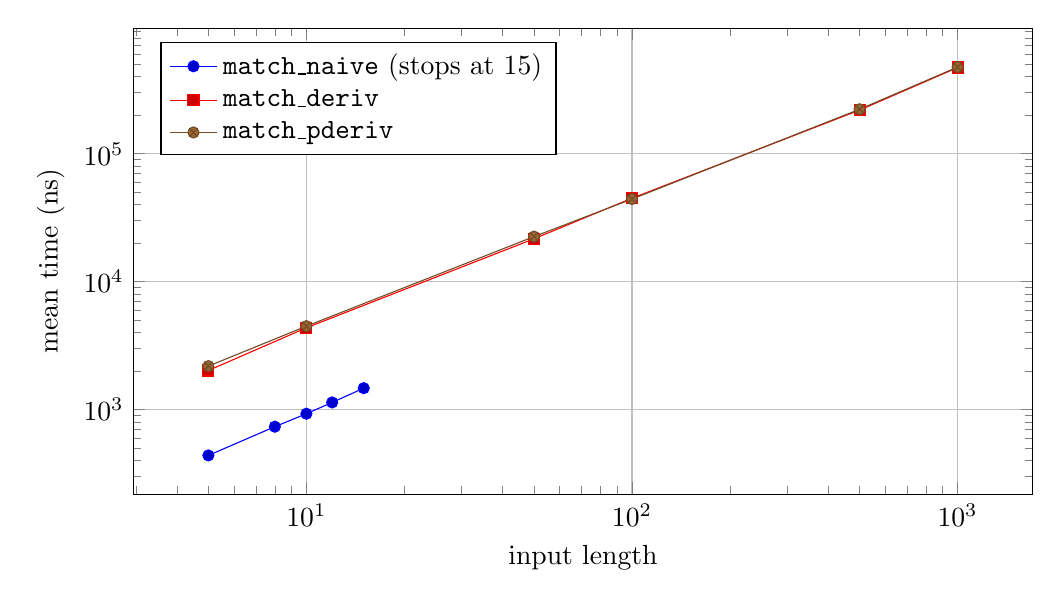
\begin{tikzpicture}
\begin{axis}[
  width=13cm, height=7.5cm,
  xlabel={input length}, ylabel={mean time (ns)},
  xmode=log, ymode=log,
  legend pos=north west, legend cell align=left,
  grid=major,
]
\addplot coordinates {(5,438.9) (8,736.1) (10,929.6) (12,1139) (15,1472)};
\addlegendentry{\texttt{match\_naive} (stops at 15)}
\addplot coordinates {(5,2024) (10,4363) (50,21653) (100,44934) (500,219540) (1000,471765)};
\addlegendentry{\texttt{match\_deriv}}
\addplot coordinates {(5,2189) (10,4495) (50,22518) (100,44276) (500,222756) (1000,476212)};
\addlegendentry{\texttt{match\_pderiv}}
\end{axis}
\end{tikzpicture}
\end{center}

%

\paragraph{Stack depth: recursive vs.\ iterative construction.}
\label{sec:stack-depth}
Comparing recursive and loop-based standard derivative parser.

%

\paragraph{Heap allocation: \texttt{deriv\_std} vs.\ \texttt{deriv\_bc}.}
\label{sec:heap-allocation} 
Savings without backward pass.

%

\paragraph{Derivative-based vs.\ partial-derivative-based.}
\label{sec:deriv-vs-pderiv-performance}

\begin{center}
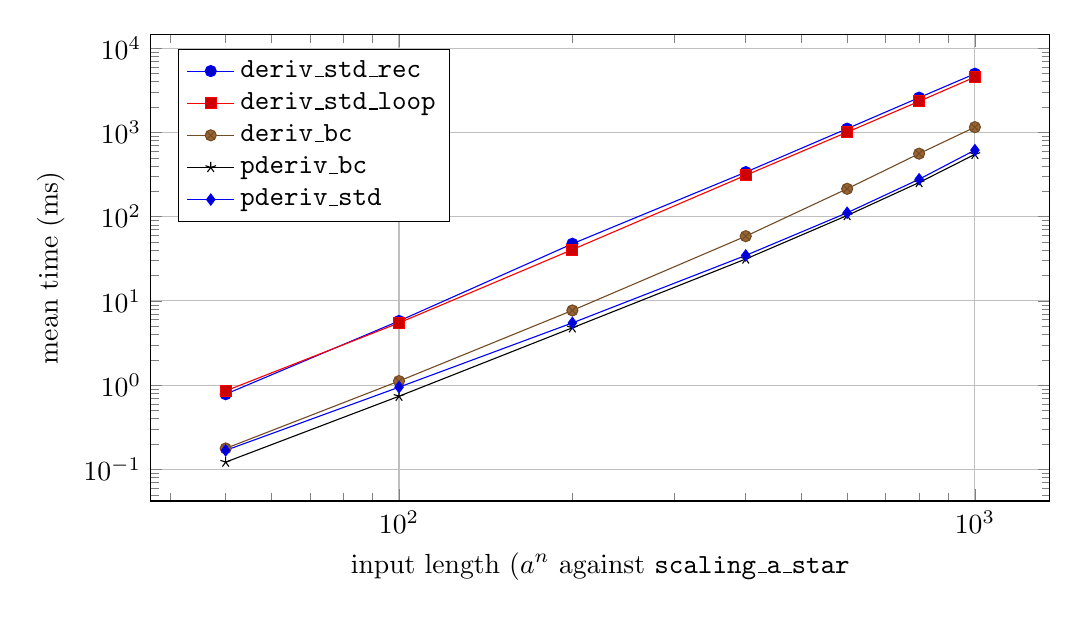
\begin{tikzpicture}
\begin{axis}[
  width=13cm, height=7.5cm,
  xlabel={input length ($a^n$ against \texttt{scaling\_a\_star}}, ylabel={mean time (ms)},
  xmode=log, ymode=log,
  legend pos=north west, legend cell align=left,
  grid=major,
]
\addplot coordinates {(50,0.781781) (100,5.782) (200,47.659) (400,337.588) (600,1108) (800,2587) (1000,4968)};
\addlegendentry{\texttt{deriv\_std\_rec}}
\addplot coordinates {(50,0.856238) (100,5.485) (200,40.639) (400,310.084) (600,1006) (800,2339) (1000,4538)};
\addlegendentry{\texttt{deriv\_std\_loop}}
\addplot coordinates {(50,0.177474) (100,1.119) (200,7.717) (400,58.650) (600,214.236) (800,559.635) (1000,1155)};
\addlegendentry{\texttt{deriv\_bc}}
\addplot coordinates {(50,0.122207) (100,0.739572) (200,4.796) (400,31.445) (600,103.264) (800,254.264) (1000,549.164)};
\addlegendentry{\texttt{pderiv\_bc}}
\addplot coordinates {(50,0.168377) (100,0.947508) (200,5.485) (400,34.691) (600,111.227) (800,278.002) (1000,616.815)};
\addlegendentry{\texttt{pderiv\_std}}
\end{axis}
\end{tikzpicture}
\end{center}

%

\paragraph{Benchmark results.}
\label{sec:benchmark-results}

\begin{center}
\begin{tabular}{lrrrr}
\hline
Parser & $n{=}5$ & $n{=}10$ & $n{=}15$ & $n{=}18$ \\
\hline
\texttt{deriv\_std\_rec} & 8.0\,\textmu s & 110.7\,\textmu s & 1.427\,ms & 6.052\,ms \\
\texttt{deriv\_bc} & 11.4\,\textmu s & 183.8\,\textmu s & 4.175\,ms & 49.491\,ms \\
\texttt{pderiv\_bc} & 13.4\,\textmu s & 210.6\,\textmu s & 2.207\,ms & 9.236\,ms \\
\texttt{pderiv\_std} & 22.4\,\textmu s & 323.9\,\textmu s & 3.374\,ms & 14.263\,ms \\
\hline
\end{tabular}
\end{center}

%
%
%

\subsection{Evaluation on the Mamouras Regex Dataset}
\label{sec:mamouras-benchmark-results}

\begin{itemize}
  \item \textbf{Corpus sample sweep}
  \item \textbf{Neutral-case probe}
  \item \textbf{Worst-case probe}
  \item \textbf{Best-case probe}
\end{itemize}


%
%
%

\section{Discussion of Results}
\label{sec:results-discussion}

\subsection{Optimization Challenges and Insights}
\label{sec:optimization-challenges}
\label{sec:further-performance-optimizations}

\paragraph{Character classes in place of literal alternation.}
\label{sec:char-class-optimization}

\paragraph{Frontier-wide deduplication.}
